% \iffalse
\let\negmedspace\undefined
\let\negthickspace\undefined
\documentclass[journal,12pt,twocolumn]{IEEEtran}
\usepackage{cite}
\usepackage{amsmath,enumitem,amssymb,amsfonts,amsthm}
\usepackage{algorithmic}
\usepackage{graphicx}
\usepackage{float}
\usepackage{textcomp}
\usepackage{xcolor}
\usepackage{caption}
\usepackage{txfonts}
\usepackage{listings}
\usepackage{enumitem}
\usepackage{mathtools}
\usepackage{gensymb}
\usepackage{comment}
\usepackage[breaklinks=true]{hyperref}
\usepackage{tkz-euclide} 
\usepackage{listings}
\usepackage{tabularx}
\usepackage{gvv}                                        
\def\inputGnumericTable{}                                 
\usepackage[latin1]{inputenc}                              
\usepackage{color}                                            
\usepackage{array}                                            
\usepackage{longtable}                                       
\usepackage{calc}                                             
\usepackage{multirow}                                         
\usepackage{hhline}                                           
\usepackage{ifthen}                                        
\usepackage{lscape}
\newtheorem{theorem}{Theorem}[section]
\newtheorem{problem}{Problem}
\newtheorem{proposition}{Proposition}[section]
\newtheorem{lemma}{Lemma}[section]
\newtheorem{corollary}[theorem]{Corollary}
\newtheorem{example}{Example}[section]
\newtheorem{definition}[problem]{Definition}
\newcommand{\BEQA}{\begin{eqnarray}}
\newcommand{\EEQA}{\end{eqnarray}}
\newcommand{\define}{\stackrel{\triangle}{=}}
\theoremstyle{remark}
\newtheorem{rem}{Remark}
\begin{document}



\bibliographystyle{IEEEtran}
\vspace{3cm}

\title{NCERT 11.9.5 26Q}
\author{EE23BTECH11015 - DHANUSH V NAYAK$^{*}$% <-this % stops a space
}
\maketitle
\newpage
\bigskip

\renewcommand{\thefigure}{\theenumi}
\renewcommand{\thetable}{\theenumi}

\bibliographystyle{IEEEtran}
\textbf{Question:} Show that
\begin{align}
    \frac{1\times2^2 + 2\times3^2 + \dots + n\times(n+1)^2}{1^2\times2 + 2^2\times3 + \dots + n^2\times(n+1)}  = \frac{3n+5}{3n+1}\notag
\end{align}
\textbf{Solution:}
\begin{table}[H]
\centering
  \renewcommand\thetable{1}
\setlength{\extrarowheight}{9pt}
\resizebox{0.54\textwidth}{!}{
\begin{tabular}{|c|c|c|}
\hline
\textbf{Parameter} & \textbf{Description} & \textbf{Value} \\ \hline
$n$ & Integer & 1, 2, 3, 4, ... \\ \hline
$x_1(n)$ & Numerator sequence & $\brak{n^{3} + 5n^{2} + 20n + 4} \cdot u\brak{n}$ \\ \hline
$x_2(n)$ & Denominator sequence & $\brak{n^{3}+4n^{2}+5n+2}\cdot u\brak{n}$ \\ \hline
$X_1(z)$ & z-transform of $x_1(n)$ & $\frac{4+14z^{-1}-24z^{-2}+12z^{-3}}{\brak{1-z^{-1}}^4} , \cbrak{z\in\mathbb{C} : \lvert z \rvert > 1} $ \\ \hline
$X_2(z)$ & z-transform of $x_2(n)$ & $\frac{2+4z^{-1}}{\brak{1-z^{-1}}^4},\cbrak{z\in\mathbb{C} : \lvert z \rvert > 1}  $ \\ \hline
$U(z)$ & z-transform of $u(n)$ & $\frac{1}{1 - z^{-1}},\cbrak{z\in\mathbb{C} : \lvert z \rvert > 1}  $ \\ \hline
ROC & Region of convergence & $\left\{ z : \left|\sum_{n=-\infty}^{\infty} x(n)z^{-n}\right| < \infty \right\}$ \\ \hline
$X_k(z)$ & z-transform of $n^k u(n)$ & $\brak{-z}^k \frac{d^kU\brak{z}}{dz^k} , \hspace{4pt}\cbrak{z\in\mathbb{C} : \lvert z \rvert > 1} $ \\ \hline
$X_1\brak{z}$ & z-transform of $n\cdot u\brak{n}$ & $\frac{z^{-1}}{\brak{1-z^{-1}}^2}  , \hspace{4pt} \cbrak{z\in\mathbb{C} : \lvert z \rvert > 1} $ \\ \hline 
$X_2\brak{z}$ & z-transform of $n^{2}\cdot u\brak{n}$ & $\frac{z^{-1}\brak{z^{-1}+1}}{\brak{1-z^{-1}}^3} , \hspace{4pt} \cbrak{z\in\mathbb{C} : \lvert z \rvert > 1} $ \\ \hline 
$X_3\brak{z}$ & z-transform of $n^{3}\cdot u\brak{n}$ & $\frac{z^{-1}\brak{1+4z^{-1}+z^{-2}}}{\brak{1-z^{-1}}^4}, \hspace{4pt} \cbrak{z\in\mathbb{C} : \lvert z \rvert > 1} $ \\ \hline 
$X_4\brak{z}$ & z-transform of $n^{4}\cdot u\brak{n}$ & $\frac{z^{-1}\brak{1+11z^{-1}+11z^{-2}+z^{-3}}}{\brak{1-z^{-1}}^5}, \hspace{4pt} \cbrak{z\in\mathbb{C} : \lvert z \rvert > 1} $ \\ \hline 
\end{tabular}}
\caption{Parameter Table}
\label{tab:11.9.5.26.1}
\end{table}

\begin{enumerate}[label=\arabic*.]
\item Consider the Numerator of the LHS part:
\begin{align}
    1\times2^2 + 2\times3^2 + \dots + n\times(n+1)^2 &= \sum_{k=1}^n k(k+1)^2 
\end{align}
\begin{align}
                       \sum_{k=1}^n k(k+1)^2    &= \left(\frac{n\brak{n+1}}{2}\right)^{\scriptstyle 2} + 2\cdot \frac{n\brak{n+1}\brak{2n+1}}{6}\\ &+\frac{n\brak{n+1}}{2}\notag 
\end{align}
\begin{align}
                          &= \frac{n\brak{n+1}\brak{n+2}\brak{3n+5}}{12}\\
    x\brak{n} &=  \frac{\brak{n+1}\brak{n+2}\brak{n+3}\brak{3n+8}}{12}\cdot u\brak{n}\\
         &= \frac{3n^4 + 26n^3 + 81n^2 + 106n + 48}{12}\cdot u\brak{n} \label{eq:11.9.5.26.1}
\end{align}
\begin{figure}[h]
    \hspace{1cm}
    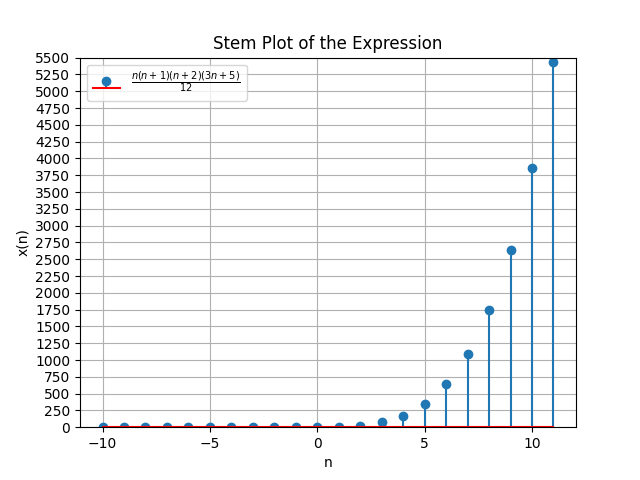
\includegraphics[width=1\columnwidth]{Figure_1.png}
    \caption{Stem Plot of $x\brak{n}$}
\end{figure}

By the differentiation property :
\begin{align}
x\brak{n} &\stackrel{\mathcal{Z}}{\longleftrightarrow} X\brak{z},\hspace{4pt} ROC = R\\
n^k x\brak{n} &\stackrel{\mathcal{Z}}{\longleftrightarrow} \brak{-z}^k \frac{d^kX\brak{z}}{dz^k},\hspace{4pt} ROC = R \\
\implies n^k u\brak{n} &\stackrel{\mathcal{Z}}{\longleftrightarrow} \brak{-z}^k \frac{d^kU\brak{z}}{dz^k}\\
    \implies X_k\brak{z} &=  \brak{-z}^k \frac{d^kU\brak{z}}{dz^k} , \hspace{4pt}ROC=|z|>1\label{eq:11.9.5.26.3} 
\end{align}
\begin{align}
X\brak{z} &= \frac{1}{12}\brak{3X_4\brak{z} + 26X_3\brak{z} + 81X_2\brak{z} + 106X_1\brak{z}} \label{eq:11.9.5.26.4} \notag \\
&\quad + 48U \brak{z} 
\end{align}
\text{Refering to table\ref{tab:11.9.5.26.1}} for $X_k$ and $U\brak{z}$ values 
\begin{align}
    X\brak{z}&= \frac{24\brak{2+z^{-1}}}{\brak{1-z^{-1}}^5} ,\hspace{4pt} ROC=|z|>1
\end{align}
\item Consider the Denominator of the RHS part:
\begin{equation}
    1^2\times2 + 2^2\times3 +\dots + n^2\times\brak{n+1} = \sum_{k=1}^n k^2\brak{k+1}
\end{equation}
\begin{align}
           \sum_{k=1}^n k^2\brak{k+1}&=  \left(\frac{n\brak{n+1}}{2}\right)^{\scriptstyle 2}+\frac{n\brak{n+1}\brak{2n+1}}{6}\\
                           &= \frac{\brak{n+1}\brak{n+2}\brak{n+3}\brak{3n+4}}{12}
\end{align}
\begin{align}
    \frac{\brak{n+1}\brak{n+2}\brak{n+3}\brak{3n+4}}{12}\cdot u\brak{n} &= y\brak{n}\label{eq:11.9.5.26.5} 
\end{align}
\begin{figure}[h]
    \hspace{1cm}
    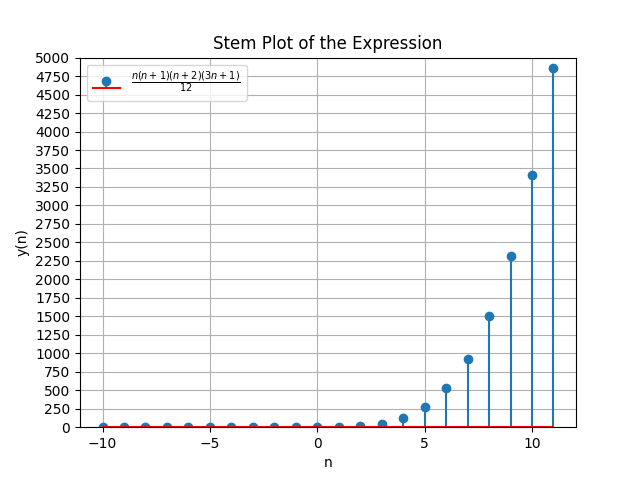
\includegraphics[width=1\columnwidth]{Figure_2.png}
    \caption{Stem Plot of $y\brak{n}$}
\end{figure}

\begin{align}
    Y\brak{z} &= \sum_{n=-\infty}^\infty y\brak{n}\cdot z^{-n}\\
    X_k&=Y_k\label{eq:11.9.5.26.6} 
\end{align}
\text{Refering to table\ref{tab:11.9.5.26.1}} for $Y_k$ and $U\brak{z}$ values 
\begin{align}
    Y\brak{z} &=\frac{1}{12}\brak{3Y_4\brak{z} + 22Y_3\brak{z} + 57Y_2\brak{z} + 62Y_1\brak{z}} \\
&\quad + 24U\brak{z} \notag 
\end{align}
\begin{align}
        Y\brak{z} &= \frac{24 \brak{1+2z^{-1}}}{\brak{1-z^{-1}}^5} ,\hspace{4pt} ROC=|z|>1
\end{align}
\end{enumerate}
\end{document}
